\ifx\mainclass\undefined
\documentclass[cn,11pt,chinese,black,simple]{elegantbook}
\usepackage{pdfpages}
% 微分号
\newcommand{\dd}[1]{\mathrm{d}#1}
\newcommand{\pp}[1]{\partial{}#1}

% FT LT ZT
\newcommand{\dtft}[1]{\text{DTFT}[#1]}
\newcommand{\dtftr}[1]{\text{DTFT}^{-1}[#1]}
\newcommand{\dtfta}{\xrightarrow{\text{DTFT}}}

\newcommand{\where}[1]{\Big|_{#1}}
\newcommand{\abs}[1]{\left| #1 \right|}
\newcommand{\zt}[1]{\mathscr{Z}[#1]}
\newcommand{\ztr}[1]{\mathscr{Z}^{-1}[#1]}
\newcommand{\zta}{\xrightarrow{\mathscr{Z}}} 
\newcommand{\lt}[1]{\mathscr{L}[#1]}
\newcommand{\lta}{\xrightarrow{\mathscr{L}}} 
\newcommand{\ft}[1]{\mathscr{F}[#1]}
\newcommand{\fta}{\xrightarrow{\mathscr{F}}} 
\newcommand{\dsum}{\displaystyle\sum}
\newcommand{\aint}{\int_{-\infty}^{+\infty} }

% 积分求和号

% 简易图片插入
\newcommand{\qfig}[3][nolabel]{
  \begin{figure}[!htb]
      \centering
      \includegraphics[width=0.6\textwidth]{#2}
      \caption{#3}
      \label{#1}
  \end{figure}
}

\usepackage{pdfpages}
\includepdfset{pagecommand=\thispagestyle{plain}}
% 表格
\renewcommand\arraystretch{1.5}

\usepackage{shapepar}
\usepackage{longtable}
% 日期

\begin{document}
\fi 
\def\chapname{review}



% Start Here

\chapter{离散信号与系统}

\section{因果性、记忆性}

是否用到了 \(x[n]\) 的未来值/过去值,而不是其他可计算的值。

\section{LTI 系统}

既是线性系统,又是时不变系统,称为LTI系统。其\textbf{充要条件}是 \(y[n] = x[n] \otimes h[n]\) 。

\subsection{因果系统}

\(h[n] = h[n] u[n]\) 

\subsection{稳定系统}

\[
\dsum_{-\infty}^{+\infty} |h(n)| =M<+\infty
\]

\subsection{特征频率与 LTI 系统}

若是有一个无限长的指数信号,那么有一个单频信号:

2.27

\[
    \left[e^{j \omega_{0} n}\right]\rightarrow \dsum_{k=-\infty}^{+\infty} 2 \pi \delta\left(\omega-\omega_{0}+2 k \pi\right)
\]

但是若是有限长,那么就有引入除去 \(\omega_0\) 的分量,因此对于一个 LTI 系统来说,放大 \(e^{j \omega_0 n}\) 和 \(e^{j \omega_0 n} u[n]\) 需要的系统函数是不一样的。

\section{差分方程的阶数}

输出 \(y[n-i]\) 最高值和最低值 \(i\) 的差值。

LCCDE = linear constant-coefficient difference equation .



\chapter{DTFT 变换}


\section{频域阶数}

2.42

若是在原有的系统函数多一个 \(z\) ,说明原来 \(a_0 z^0\) 的位置变成了 \(a_0 z^1\) ,也就是 \(a_n\) 变成了 \(a_{n+1}\) 。 同理 \(z^{-1}\) 对应 \(a_{n-1}\) 。由于使用因果信号, \(z^{-1}\) 的形式更合适。

\section{系统设计}

2.56 ,

需要一个系统时,可以通过其定义入手,配凑式子。 同时,对于特定的频率分量,其幅度、角度变换是由其频率响应改变的。

\section{DTFT 推导细节}

\[
\begin{aligned}
D T F T^{-1}\left[X\left(e^{j \omega}\right)\right]&=\dfrac{1}{2 \pi} \int_{-\pi}^{\pi} X\left(e^{j \omega}\right) e^{j \omega n} d \omega \\
&=\dfrac{1}{2 \pi} \int_{-\pi}^{\pi}\left(\dsum_{k=-\infty}^{+\infty} x(k) e^{-j \omega k}\right) e^{j \omega n} d \omega \\
&=\dsum_{k=-\infty}^{+\infty} x(k) \dfrac{1}{2 \pi} \int_{-\pi}^{\pi} e^{-j \omega(k-n)} d \omega\\
&=\dsum_{k=-\infty}^{+\infty} x(k) \delta(k-n)=x(n)
\end{aligned}
\]

注意  \(2\pi\) 与 \(\delta(n)\) 的由来:单位虚数的积分。

将 IDTFT 展开成累加的形式,实际上是将不同频率的分量逐个恢复:

\begin{align*}
    \begin{array}{l}
    X(n)=\dfrac{1}{2 \pi} \int_{-\pi}^{\pi} X\left(e^{j \omega}\right) e^{j \omega n} d \omega \\
    =\dfrac{1}{2 \pi} \dsum_{-\infty}^{+\infty} X\left(e^{j k \Delta \omega}\right) e^{j k \Delta \omega n} \Delta \omega=\dsum_{-\infty}^{+\infty} \dfrac{\left[X\left(e^{j k \Delta \omega}\right) \Delta \omega\right]}{2 \pi} e^{j k \Delta \omega n}
    \end{array}
\end{align*}



\begin{longtable}{ll} 
    \caption{DTFT 变换对} \\ 
    \toprule
    时域函数 & DTFT  \\
    \midrule
    \endfirsthead
    
    \toprule
    时域函数 & DTFT  \\
    \midrule
    \endhead 
  
    \hline
    \multicolumn{2}{c}{见下页}\\   \bottomrule
    \endfoot
  
    \bottomrule
    \endlastfoot
    \(\delta(n)\) & 1\\
    \(1\) & \(\dsum_{k=-\infty}^{+\infty} 2 \pi \delta(\omega+2 k \pi)\) \\ 
    \(u(n)\) & \(\dfrac{1}{1-e^{-j \omega}}+\dsum_{k=-\infty}^{+\infty} \pi \delta(\omega+2 k \pi)\)  \\
    \(e^{j\omega_0 n}\) & \(
        \dsum_{k=-\infty}^{+\infty} 2 \pi \delta\left(\omega-\omega_{0}+2 k \pi\right)
        \)\\
    \(W_N(n)\) & \(\dfrac{\sin \left(\dfrac{\omega N}{2}\right)}{\sin \left(\dfrac{\omega}{2}\right)} e^{-j \dfrac{(N-1) \omega}{2}}\) \\
    \(\dfrac{w_{c}}{\pi} \dfrac{\sin \left[w_{c}(n-\alpha)\right]}{w_{c}(n-\alpha)}\)  & \(e^{-j\omega\alpha} (u(\omega+\omega_c) - u(\omega-\omega_c))\)\\ 
\end{longtable}


\begin{longtable}{ll} 
    \caption{DTFT 变换性质} \\ 
    \toprule
    性质名称 & 表达式  \\
    \midrule
    \endfirsthead
    
    \toprule
    性质名称 & 表达式  \\
    \midrule
    \endhead 
  
    \hline
    \multicolumn{2}{c}{见下页}\\   \bottomrule
    \endfoot
  
    \bottomrule
    \endlastfoot
    线性 & \\ 
    时域平移-频域调制 &  \(x(n-m) \rightarrow e^{-j w m} X\left(e^{j w}\right)\) \\
    时域调制-频域平移 & \(e^{j n w} x(n) \quad \rightarrow  X\left(e^{j\left(w-w_{0}\right)}\right)\) \\ 
    时域翻折 & \(x(-n) \rightarrow X(e^{-j \omega})\) \\ 
    帕塞瓦尔定理 & \(\begin{aligned}
        \dsum_{n=-\infty}^{\infty} x(n) y^{*}(n) &=\dfrac{1}{2 \pi} \int_{-\pi}^{\pi} X\left(e^{j w}\right) Y^{*}\left(e^{j w}\right) d w \\
        \dsum_{n=-\infty}^{\infty}|x(n)|^{2}&=\dfrac{1}{2 \pi} \int_{-\pi}^{\pi}\left|X\left(e^{j w}\right)\right|^{2} d w
        \end{aligned}\) \\
\end{longtable}

可以利用帕赛瓦尔定理解决一些求和式子:Slide P83.



\section{DTFT 对称性}

共轭对称与共轭反对称序列定义,实际上是实部、虚部分别的奇偶对称: \[
    \begin{array}{l}
    x_{e}(n)=x_{e}^{*}(-n) \\
    x_{o}(n)=-x_{o}^{*}(-n)
    \end{array}
\]

任意序列都可以进行共轭分解:

\[\begin{aligned}
    x(n) &= x_e(n) + x_o(n) \\ 
    x(-n) &= x_e(-n) + x_o(-n) = x_e^*(n) - x_o^*(n) 
\end{aligned}\]

\[
\begin{array}{l}
x_{e}(n)=\frac{1}{2}\left[x(n)+x^{*}(-n)\right] \\
x_{o}(n)=\frac{1}{2}\left[x(n)-x^{*}(-n)\right]
\end{array}
\]

根据下一小节的性质:

\[
\begin{array}{l}
X_{e}\left(e^{j \omega}\right)=\frac{1}{2}\left[X\left(e^{j \omega}\right)+X^{*}\left(e^{-j \omega}\right)\right] \\
X_{o}\left(e^{j \omega}\right)=\frac{1}{2}\left[X\left(e^{j \omega}\right)-X^{*}\left(e^{-j \omega}\right)\right]
\end{array}
\]

同样的对频域函数进行变换:

\[X(e^{j\omega}) = X_e(e^{j\omega}) + X_o(e^{-j\omega})\] 

\[
\begin{array}{l}
X_{e}\left(e^{j \omega}\right)=\frac{1}{2}\left[X\left(e^{j \omega}\right)+X^{*}\left(e^{-j \omega}\right)\right] \\
X_{o}\left(e^{j \omega}\right)=\frac{1}{2}\left[X\left(e^{j \omega}\right)-X^{*}\left(e^{-j \omega}\right)\right]
\end{array}
\]

逆变换:
\[
\begin{array}{l}
D T F T\{\operatorname{Re}[x(n)]\}=X_{e}\left(e^{j \omega}\right) \\
D T F T\{j \operatorname{Im}[x(n)]\}=X_{o}\left(e^{j \omega}\right)
\end{array}
\]
\section{变换共轭性质}

具有普适性。

\[
\begin{array}{c}
\mathcal{Z}\left[x^{*}[n]\right]=\dsum_{n=-\infty}^{\infty} x^{*}[n] z^{-n}=\left(\dsum_{n=-\infty}^{\infty} x[n]\left(z^{*}\right)^{-n}\right)^{*}=X^{*}\left(z^{*}\right) \\
\mathcal{Z}[x[-n]]=\dsum_{n=-\infty}^{\infty} x[-n] z^{-n}=\dsum_{n=-\infty}^{\infty} x[n]\left(z^{-1}\right)^{-n}=X\left(z^{-1}\right) \\
\mathcal{Z}[\operatorname{Re}\{x[n]\}]=\mathcal{Z}\left[\dfrac{x[n]+x^{*}[n]}{2}\right]=\dfrac{1}{2}\left[X(z)+X^{*}\left(z^{*}\right)\right] \\
\mathcal{Z}[\operatorname{Im}\{x[n]\}]=\mathcal{Z}\left[\dfrac{z[n]-x^{*}[n]}{2 j}\right]=\dfrac{1}{2 j}\left[X(z)-X^{*}\left(z^{*}\right)\right]
\end{array}
\]

\section{Z 变换}


\begin{longtable}{lll} 
    \caption{\(\mathscr{Z}\)变换对} \\ 
    \toprule
    时域函数 & \(z\)域函数 & ROC \\
    \midrule
    \endfirsthead
    
    \toprule
    时域函数 & \(z\)域函数 & ROC \\
    \midrule
    \endhead 
  
    \hline
    \multicolumn{3}{c}{见下页}\\   \bottomrule
    \endfoot
  
    \bottomrule
    \endlastfoot
    \(\delta(n)\) & 1 & 全平面\\
    \(u(n)\) & \(\dfrac{z}{z-1}\) & \(\abs{z}>1\) \\
    \(a^n u(n)\) & \(\dfrac{z}{z-a}\) & \(\abs{z}>a\) \\
    \(-a^n u(-n-1)\) & \(\dfrac{z}{z-a}\) & \(\abs{z}<a\)\\
    \(\cos(\omega_0 n)u(n)\) & \(\dfrac{z^2-z \cos \omega_0}{z^2 - 2 z \cos\omega_0 + 1}\) & \(\abs{z}>1\) \\
    \(\sin(\omega_0 n)u(n)\) & \(\dfrac{z \sin\omega_0}{z^2 -2 z \cos\omega_0 + 1}\) &  \(\abs{z}>1\) \\

\end{longtable}
  


\begin{longtable}{llll} 
    \caption{\(\mathscr{Z}\)变换性质} \\ 
    \toprule
    时域函数 & \(z\)域函数 & 原ROC  & 变换后ROC\\
    \midrule
    \endfirsthead
    
    \toprule
    时域函数 & \(z\)域函数 & 原ROC  & 变换后ROC\\
    \midrule
    \endhead 
  
    \hline
    \multicolumn{4}{c}{见下页}\\   \bottomrule
    \endfoot
  
    \bottomrule
    \endlastfoot
    \(x(-n)\) & \(X(z^{-1})\) & \(\alpha < \abs{z} < \beta\) & \(\dfrac{1}{\beta} < \abs{z} < \dfrac{1}{\alpha}\)\\
    \(x(\dfrac{n}{a}),a>0\) & \(X(z^a)\) & \(\alpha < \abs{z} < \beta\) & \(\alpha^{1/a} < \abs{z} < \beta^{1/a}\) \\
    \(x(n \pm m)\) & 双边 \(z^{\pm m}X(z)\) &  \(\alpha < \abs{z} < \beta\) &  \(\alpha < \abs{z} < \beta\) \\
    \(x(n - m)u(n)\) & 单边 \(z^{-m} \left[X(z) + \dsum_{k=-m}^{-1}x(k)z^{-k}\right]\) & \(\abs{z} > a\) & \(\abs{z} > a\) \\
    \(x(n + m)u(n)\) & 单边 \(z^{m} \left[X(z) - \dsum_{k=0}^{m-1}x(k)z^{-k}\right]\) & \(\abs{z} > a\) & \(\abs{z} > a\) \\
    线性性 & & & 原收敛域的交集 \\
    \(n x(n)\) & \(-z \dfrac{\dd{X(z)}}{\dd{z}}\) & \(\alpha < \abs{z} < \beta\) & \(\alpha < \abs{z} < \beta\)\\
    \(n^m x(n)\) & \(\left[-z\dfrac{\dd{}}{\dd{z}}\right]^m X(z)\) & \(\alpha < \abs{z} < \beta\) & \(\alpha < \abs{z} < \beta\)\\
    \(a^n x(n)\) & \(X(\dfrac{z}{a})\) &  \(\alpha < \abs{z} < \beta\) &  \(\alpha < \abs{\dfrac{z}{a}} < \beta\) \\
    \(x_1(n) \otimes x_2(n)\) & \(X_1(z) X_2(z)\) & & 原收敛域交集 \\
    \(x_1(n)x_2(n)\) & \(\dfrac{1}{2 \pi j}\displaystyle\oint_C X_1(\dfrac{z}{v})X_2(v) v^{-1} \dd{v} \)\footnote{其中\(C\)是\(X_1(\dfrac{z}{v})X_2(v)\) 收敛域交集内的逆时针方向围线} & & 收敛域是边界的乘积 \\
\end{longtable}

初值定理 \[\lim _{z \rightarrow \infty} X(z)=\lim _{z \rightarrow \infty} \dsum_{n=0}^{\infty} x(n) z^{-n}=x(0)\]

终值定理 \[\lim_{z\rightarrow 1}(z-1)X(z) = x(\infty)\]

帕塞瓦尔定理

\[
\left.Y(z)\right|_{z=1}=\sum_{n=-\infty}^{+\infty} x(n) h^{*}(n)=\frac{1}{2 \pi j} \oint_{c} X(v) H^{*}\left(\frac{1}{V^{*}}\right)_{V}^{-1} d V
\]

\section{逆 Z 变换}

\subsection{部分分式法}

对于有理多项式 \[
    X(z)=\dfrac{B(z)}{A(z)}=\dfrac{b_{m} z^{m}+b_{m-1} z^{m-1}+\cdots+b_{1} z+b_{0}}{a_{n} z^{n}+a_{n-1} z^{n-1}+\cdots+a_{1} z+a_{0}}
\]
对于分解得到的 \(\dfrac{k z}{z-a}\)

\[
\begin{aligned}
    &k a^n u(n), \abs{z} > a\\
    &-k a^n u(-n-1), \abs{z} < a\\
\end{aligned}    
\]

\section{从能量看 Z 变换与 DTFT} 

时域频域的能量是一致的,没有发生衰减。


\section{Z 变换与时域频域}

为了解决非零状态系统,使用单边 Z 变换。

系统不改变频率:

\[
\begin{array}{l}
y(n)=x(n)^{*} h(n) \\
=\sum_{m=-\infty}^{+\infty} h(m) e^{j\left[\omega_{0}(n-m)+\phi\right]}=e^{j\left[\omega_{0} n+\phi\right]} \sum_{m=-\infty}^{+\infty} h(m) e^{-j \omega_{0} m} \\
=e^{j\left[\omega_{0} n+\phi\right]} H\left(e^{j \omega_{0}}\right)=x(n) H\left(e^{j \omega_{0}}\right)
\end{array}
\]

\section{系统零极点与频率响应}

\textbf{单位圆}上的系统函数是频率响应。

\subsection{幅度响应}

\begin{itemize}
    \item 原点处的零极点幅度无影响
    \item 经过单位圆上的零点幅度归零,单位圆附近的零点出现谷点
    \item 经过单位圆上的极点幅度无穷大,单位圆附近的极点出现峰点
    \item 远离零极点时影响较小
\end{itemize}

\subsection{相位响应}

\begin{itemize}
    \item 原点处的零极点对相位影响为线性,极点会引起滞后,零点会引起超前
    \item 靠近单位圆的零极点会引起较大的波动
    \item 远离极点零点的位置变换比较平缓
    \item 单位圆外部零点或极点造成相位连续增长,而单位圆内零极点对相位影响则随频率周期性归零
\end{itemize}

对于圆内外零极点:

\begin{itemize}
    \item 圆内极点:顺时针经过,相位迅速延后
    \item 圆外极点:顺时针经过,相位迅速提前
    \item 圆内零点:顺时针经过:相位迅速提前
    \item 圆外零点:顺时针经过:相位迅速延后
\end{itemize}

过单位圆零点相位突变 \(\pi\) 。

\section{LTI 系统幅相特性分析}

当给定幅度特性时,总可以通过共轭分解找到一个系统满足要求:
 

\[
\left|H\left(e^{j \omega}\right)\right|^{2}=H\left(e^{j \omega}\right) H *\left(e^{j \omega}\right)=\left.H(z) H^{*}\left(\frac{1}{z^{*}}\right)\right|_{z=e^{j \omega}}
\]

\subsection{全通系统}

频响恒为 \(1\) ,其零极点分别为 \(a\) 与 \(1/a^*\): 

\[
H_{a p}(z)=\frac{z^{-1}-a^{*}}{1-a z^{-1}}=-a^{*}\left(\frac{z-\frac{1}{a^{*}}}{z-a}\right)
\]

其相位响应为:



\subsection{}

\chapter{复习题}

2.44,

\appendix

\chapter{零极点幅度相位研究}

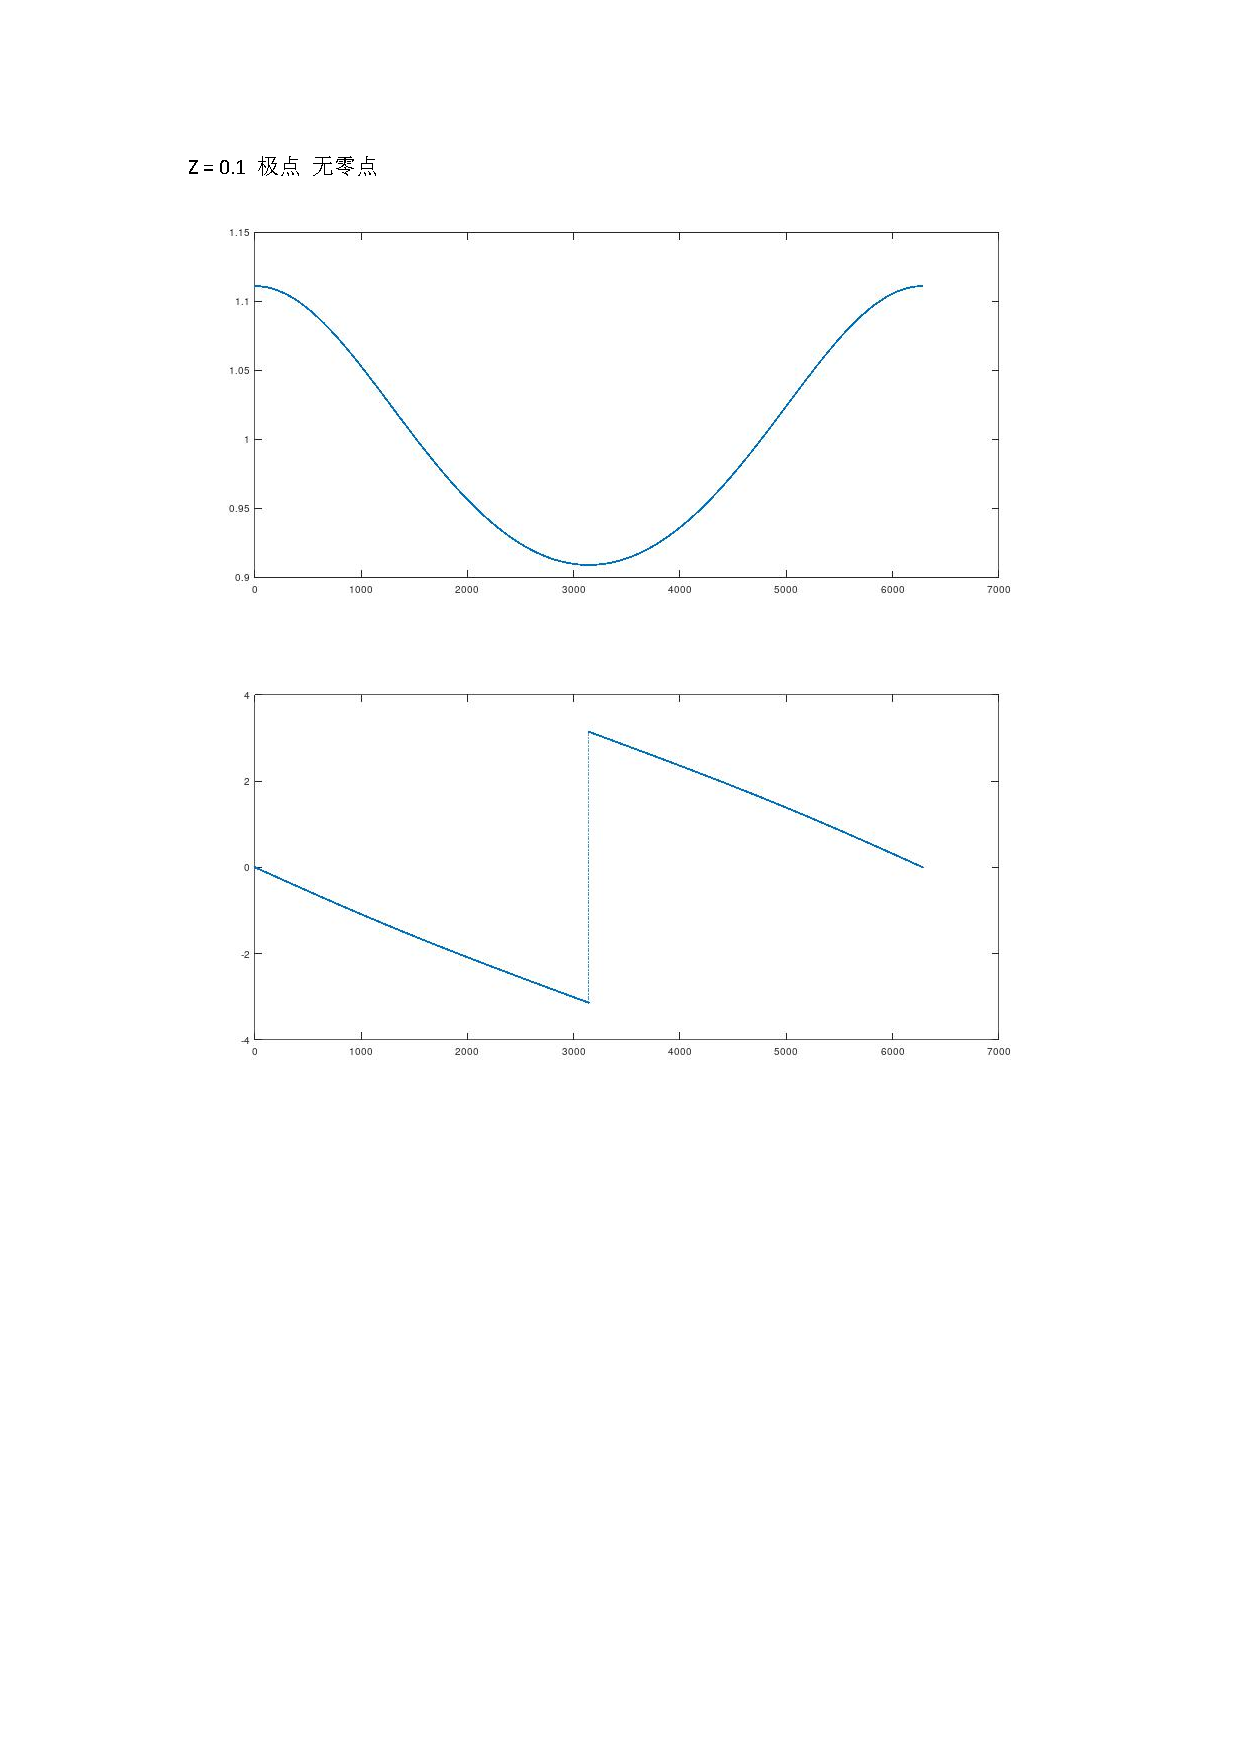
\includepdf[pages=-, pagecommand={}]{../figure/zp.pdf}
% End Here

\let\chapname\undefined
\ifx\mainclass\undefined
\end{document}
\fi  